\begin{name}
	{\tenchude}{\tendethi}{LỚP TOÁN THẦY PHÁT}{\thoigian}
\end{name}
\setcounter{ex}{0}
\Opensolutionfile{ans}[ans/ans-2-TT-26-SGDHaTinh-23]

\begin{ex}%[Đề thi thử TN Hà Tĩnh 2023]%[An Le - Ex6]%[2D4Y1-2]
	Trên mặt phẳng tọa độ, điểm biểu diễn của số phức $z=2+3i$ có tọa độ là
	\choice
	{\True $(2;3)$}
	{$(2;-3)$}
	{$(3;2)$}
	{$(3;-2)$}
	\loigiai{
		Điểm biểu diễn số phức $z=2+3i$ là $M (2;3)$.
	}
\end{ex}

\begin{ex}%[Đề thi thử TN Hà Tĩnh 2023]%[An Le - Ex6]%[2D2Y4-2]
	Đạo hàm của hàm số $y=7^x$ là
	\choice
	{$y'=x7^{x-1}$}
	{\True $y'=7^x\ln 7$}
	{$y'=\dfrac{7^x}{\ln 7}$}
	{$y'=7^x$}
	\loigiai{
		Ta có $y'=7^x\ln 7$.
	}
\end{ex}

\begin{ex}%[Đề thi thử TN Hà Tĩnh 2023]%[An Le - Ex6]%[2D2Y4-1]
	Tập xác định của hàm số $y=\log_3x$ là
	\choice
	{$\mathscr{D}=[0;+\infty)$}
	{\True $\mathscr{D}=(0;+\infty)$}
	{$\mathscr{D}=(-\infty;0)$}
	{$\mathscr{D}=(-\infty;0]$}
	\loigiai{
		Tập xác định của hàm số $y=\log_3x$ là $\mathscr{D}=(0;+\infty)$.
	}
\end{ex}

\begin{ex}%[Đề thi thử TN Hà Tĩnh 2023]%[An Le - Ex6]%[2D2Y6-1]
	Tập nghiệm của bất phương trình $3^x \leq 27$ là
	\choice
	{$[3;+\infty)$}
	{$(3;+\infty)$}
	{\True $(-\infty;3]$}
	{$(-\infty;9]$}
	\loigiai{
		Ta có $3^x \leq 27 \Leftrightarrow x \leq 3$.
	}
\end{ex}

\begin{ex}%[Đề thi thử TN Hà Tĩnh 2023]%[An Le - Ex6]%[1D3Y3-3]
	Cho cấp số cộng $(u_n)$ với $u_2=2$ và công sai $d=-3$. Giá trị của $u_3$ bằng
	\choice
	{$-5$}
	{$-6$}
	{\True $-1$}
	{$5$}
	\loigiai{
		Ta có $u_3 = u_2 + d = 2 - 3 = -1.$
	}
\end{ex}

\begin{ex}%[Đề thi thử TN Hà Tĩnh 2023]%[An Le - Ex6]%[2H3Y3-1]
	Trong KG $Oxyz$, véc-tơ $\overrightarrow{a}=2\overrightarrow{i}-3\overrightarrow{j}-\overrightarrow{k}$, với $\overrightarrow{i};\overrightarrow{j};\overrightarrow{k}$ là các véc-tơ đơn vị. Khi đó tọa độ của $\overrightarrow{a}$ là
	\choice
	{\True $\overrightarrow{a}=(2;-3;-1)$}
	{$\overrightarrow{a}=(2;3;1)$}
	{$\overrightarrow{a}=(-2;3;1)$}
	{$\overrightarrow{a}=(2;3;-1)$}
	\loigiai{
		Ta có $\overrightarrow{a}=2\overrightarrow{i}-3\overrightarrow{j}-\overrightarrow{k} \Rightarrow  \overrightarrow{a}=(2;-3;-1).$
	}
\end{ex}

\begin{ex}%[Đề thi thử TN Hà Tĩnh 2023]%[An Le - Ex6]%[2D1Y5-3]
	Cho hàm số $y=f(x)$ có bảng biến thiên như hình vẽ. Số nghiệm của phương trình $f(x)=0$ là
	\begin{center}
		\begin{tikzpicture}
			\tkzTabInit[nocadre=false,lgt=1.2,espcl=2.5,deltacl=0.6]
			{$x$/0.7, $f’(x)$/0.7, $f(x)$/2}
			{$-\infty$, $-2$, $0$, $2$, $+\infty$}
			\tkzTabLine{,-,0,+,0,-,0,+,}
			\tkzTabVar{+/ $+\infty$, -/ $-2$, +/ $1$, -/ $-2$ , +/ $+\infty$} cột 2
		\end{tikzpicture}
	\end{center}	
	\choice
	{\True $4$}
	{$3$}
	{$2$}
	{$0$}
	\loigiai{
		Ta có $f(x)=0$. Số nghiệm của phương trình là số giao điểm của đồ thị hàm số $y=f(x)$ và đường thẳng $y=0$.\\ 
		Mà $-2<0<1$ nên số nghiệm thực của phương trình $f(x)=0$ là $4$.
	}
\end{ex}

\begin{ex}%[Đề thi thử TN Hà Tĩnh 2023]%[An Le - Ex6]%[2D3Y2-1]
	Nếu $\displaystyle\int\limits_0^1 f(x)\mathrm{\,d}x=4$ và $\displaystyle\int\limits_0^1 g(x)\mathrm{\,d}x=-2$ thì $I=\displaystyle\int\limits_0^1 [f(x)+g(x)]\mathrm{\,d}x$ bằng
	\choice
	{$6$}
	{$-6$}
	{$-2$}
	{\True $2$}
	\loigiai{
		Ta có $\displaystyle\int\limits_0^1 [f(x)+g(x)]\mathrm{\,d}x=\displaystyle\int\limits_0^1 f(x)\mathrm{\,d}x+\displaystyle\int\limits_0^1 g(x)\mathrm{\,d}x=4+(-2)=2$.
	}
\end{ex}

\begin{ex}%[Đề thi thử TN Hà Tĩnh 2023]%[An Le - Ex6]%[2H3Y1-3]
	Trong KG $Oxyz$, cho mặt cầu $(S)$ tâm $I(-1;2;-3)$, bán kính $R=2$. Phương trình của mặt cầu $(S)$ là
	\choice
	{\True $(x+1)^2+(y-2)^2+(z+3)^2=4$}
	{$(x+1)^2+(y-2)^2+(z+3)^2=2$}
	{$(x-1)^2+(y-2)^2+(z-3)^2=4$}
	{$(x-1)^2+(y+2)^2+(z-3)^2=4$}
	\loigiai{
		Mặt cầu $(S)$ tâm $I(-1;2;-3)$, bán kính $R=2$ nên phương trình của $(S)$ là $(x+1)^2+(y-2)^2+(z+3)^2=4$.
	}
\end{ex}

\begin{ex}%[Đề thi thử TN Hà Tĩnh 2023]%[An Le - Ex6]%[2H3Y1-1]
	Trong KG $Oxyz$, hình chiếu vuông góc của điểm $M(1;2;3)$ lên mặt phẳng $(Oxy)$ có tọa độ
	\choice
	{\True $(1;2;0)$}
	{$(1;0;3)$}
	{$(0;2;3)$}
	{$(0;0;3)$}
	\loigiai{
		Hình chiếu vuông góc của điểm $M(1;2;3)$ lên mặt phẳng $(Oxy)$ là $(1;2;0)$.
	}
\end{ex}

\begin{ex}%[Đề thi thử TN Hà Tĩnh 2023]%[An Le - Ex6]%[2H1Y3-2]
	Thể tích của khối hộp chữ nhật có độ dài ba cạnh $2$; $3$; $4$ bằng
	\choice
	{$8$}
	{\True $24$}
	{$12$}
	{$4$}
	\loigiai{
		Thể tích của khối hộp chữ nhật là $V= 2 \cdot 3  \cdot 4 = 24$.
	}
\end{ex}

\begin{ex}%[Đề thi thử TN Hà Tĩnh 2023]%[An Le - Ex6]%[2H1Y3-2]
	Cho khối chóp $S.ABCD$ có đáy là hình chữ nhật, $AB=2$; $BC=3$; $SA$ vuông góc với đáy và $SA=5$. Thể tích khối chóp đã cho bằng
	\choice
	{$30$}
	{\True $10$}
	{$6$}
	{$2$}
	\loigiai{
		Thể tích của khối chóp là $V=\dfrac{2}{3}\cdot SA\cdot AB\cdot BC= \dfrac{1}{3} \cdot 5  \cdot 2 \cdot 3= 10$.
	}
\end{ex}

\begin{ex}%[Đề thi thử TN Hà Tĩnh 2023]%[An Le - Ex6]%[2H3Y1-3]
	Trong KG $Oxyz$, cho mặt cầu $(S) \colon (x-1)^2+(y+2)^2+(z-3)^2=16$. Điểm nào sau đây nằm bên trong mặt cầu?
	\choice
	{$N(-1;2;3)$}
	{$P(-1;2;-3)$}
	{\True $M(1;-2;1)$}
	{$Q(1;-2;-1)$}
	\loigiai{
		Ta có $(1-1)^2+(-2+2)^2+(1-3)^2<16$ suy ra điểm $M(1;-2;1)$ nằm trong mặt cầu.
	}
\end{ex}

\begin{ex}%[Đề thi thử TN Hà Tĩnh 2023]%[An Le - Ex6]%[2D4Y1-1]
	Cho số phức $z=3+4i$, mô-đun của số phức $z$ bằng
	\choice
	{\True $5$}
	{$3$}
	{$4$}
	{$7$}
	\loigiai{
		Ta có $|z|=\sqrt{3^2+4^2} = 5$.
	}
\end{ex}

\begin{ex}%[Đề thi thử TN Hà Tĩnh 2023]%[An Le - Ex6]%[2H2Y1-2]
	Cho hình nón có bán kính đáy $r$, chiều cao $h$ và độ dài đường sinh $\ell$. Đẳng thức nào sau đây đúng?
	\choice
	{$r^2=h^2+\ell^2$}
	{$h^2=r^2+\ell^2$}
	{$h=\ell$}
	{\True $\ell^2=r^2+h^2$}
	\loigiai{
		Đẳng thức $\ell^2=r^2+h^2$ đúng.
	}
\end{ex}

\begin{ex}%[Đề thi thử TN Hà Tĩnh 2023]%[An Le - Ex6]%[2H3Y3-1]
	Trong KG $Oxyz$, cho đường thẳng $d \colon \dfrac{x+1}{2}=\dfrac{y-2}{1}=\dfrac{z-1}{-2}$. Một véc-tơ chỉ phương của $d$ là
	\choice
	{$\overrightarrow{v}=(-1;2;1)$}
	{$\overrightarrow{v}=(2;1;2)$}
	{$\overrightarrow{v}=(1;-2;-1)$}
	{\True $\overrightarrow{v}=(2;1;-2)$}
	\loigiai{
		Một véc-tơ chỉ phương của $d \colon \dfrac{x+1}{2}=\dfrac{y-2}{1}=\dfrac{z-1}{-2}$ là $\overrightarrow{v}=(2;1;-2)$.
	}
\end{ex}

\begin{ex}%[Đề thi thử TN Hà Tĩnh 2023]%[An Le - Ex6]%[2D1Y2-2]
	Cho hàm số $y=f(x)$ có bảng biến thiên như hình vẽ. Hàm số đạt cực đại tại
	\begin{center}
		
\begin{tikzpicture}
			\tkzTabInit[nocadre=false,lgt=1.2,espcl=2.5,deltacl=0.6]
			{$x$/0.7, $f’(x)$/0.7, $f(x)$/2}
			{$-\infty$, $2$, $4$, $+\infty$}
			\tkzTabLine{,+,0,-,0,+,}
			\tkzTabVar{-/ $-\infty$, +/ $3$, -/ $-2$ , +/ $+\infty$}
		\end{tikzpicture}
	\end{center}
	\choice
	{\True $x=2$}
	{$x=3$}
	{$x=4$}
	{$x=-2$}
	\loigiai{
		Hàm số đạt cực đại tại $x=2$.
	}
\end{ex}

\begin{ex}%[Đề thi thử TN Hà Tĩnh 2023]%[An Le - Ex6]%[1D2Y2-1]
	Cho một nhóm học sinh có 10 bạn. Có bao nhiêu cách chọn 3 bạn để đi tình nguyện?
	\choice
	{$720$}
	{$6$}
	{\True $120$}
	{$30$}
	\loigiai{
		Số cách chọn 3 bạn trong nhóm 10 bạn là $\mathrm{C}_{10}^3=120$.
	}
\end{ex}

\begin{ex}%[Đề thi thử TN Hà Tĩnh 2023]%[An Le - Ex6]%[2D3Y1-1]
	Hàm số nào sau đây là một nguyên hàm của hàm số $f(x)=2x+3$?
	\choice
	{$F(x)=2$}
	{$F(x)=x^2+3$}
	{\True $F(x)=x^2+3x$}
	{$F(x)=2x^2+3$}
	\loigiai{
		Ta có $\displaystyle\int {f\left(x\right)}\mathrm{\,d}x=\displaystyle\int {\left(2x+3\right)}\mathrm{\,d}x=x^2+3x+C$.
	} 
\end{ex}

\begin{ex}%[Đề thi thử TN Hà Tĩnh 2023]%[An Le - Ex6]%[2D3Y2-1]
	Nếu $\displaystyle\int\limits_0^3 f(x)\mathrm{\,d}x=2$ thì $\displaystyle\int\limits_0^3 [f(x)+1]\mathrm{\,d}x$ bằng
	\choice
	{$3$}
	{$2$}
	{\True $5$}
	{$1$}
	\loigiai{
		Ta có $\displaystyle\int\limits_0^3 [f(x)+1]\mathrm{\,d}x = \displaystyle\int\limits_0^3 f(x)\mathrm{\,d}x + \displaystyle\int\limits_0^3 \mathrm{\,d}x = 2 + 3 = 5$.
	}
\end{ex}

\begin{ex}%[Đề thi thử TN Hà Tĩnh 2023]%[An Le - Ex6]%[2D3Y1-2]
	Tìm họ nguyên hàm của hàm số $f(x)=\sin 2x$.
	\choice
	{\True $\displaystyle\int{f(x)\mathrm{d}x}=-\dfrac{1}{2}\cos 2x+C$}
	{$\displaystyle\int{f(x)\mathrm{d}x}=-\cos 2x+C$}
	{$\displaystyle\int{f(x)\mathrm{d}x}=\dfrac{1}{2}\sin 2x+C$}
	{$\displaystyle\int{f(x)\mathrm{d}x}=-\sin 2x+C$}
	\loigiai{
		Ta có $\displaystyle\int{f(x)\mathrm{d}x}=-\dfrac{1}{2}\cos 2x+C$.
	}
\end{ex}

\begin{ex}%[Đề thi thử TN Hà Tĩnh 2023]%[An Le - Ex6]%[2D1Y3-1]
	Tìm giá trị lớn nhất của hàm số $y=\dfrac{x+2}{x}$ trên đoạn $\left[1;2\right]$.
	\choice
	{$\max\limits_{\left[1;2 \right]} y=2$}
	{\True $\max\limits_{\left[1;2 \right]} y=3$}
	{$\max\limits_{\left[1;2 \right]} y=\dfrac{1}{2}$}
	{$\max\limits_{\left[1;2 \right]} y=\dfrac{3}{2}$}
	\loigiai{
		Ta có $y'=-\dfrac{2}{x^2}<0$, $\forall x\in[1;2]$ nên hàm số nghịch bến trên $[1;2]$.\\
		Suy ra $\max\limits_{\left[1;2 \right]} y=y(1)=3$.
	}
\end{ex}

\begin{ex}%[Đề thi thử TN Hà Tĩnh 2023]%[An Le - Ex6]%[2D2Y3-2]
	Với $a$ là số thực dương tùy ý, $\log_3\left(3a^4\right)$ bằng
	\choice
	{$3+\log_3a$}
	{$4\log_3a$}
	{$3+4\log_3a$}
	{\True $1+4\log_3a$}
	\loigiai{
		Ta có $\log_3\left(3a^4\right)=\log_33+\log_3a^4=1+4\log_3a$.
	}
\end{ex}

\begin{ex}%[Đề thi thử TN Hà Tĩnh 2023]%[An Le - Ex6]%[2D1B5-1]
	\immini{Đường cong trong hình vẽ bên là đồ thị của hàm số nào dưới đây?
		\choice
		{$y=x^4-x^2+2$}
		{$y=-x^3-3x+2$}
		{$y=x^2-3x+2$}
		{\True $y=x^3-3x+2$}}
	{
		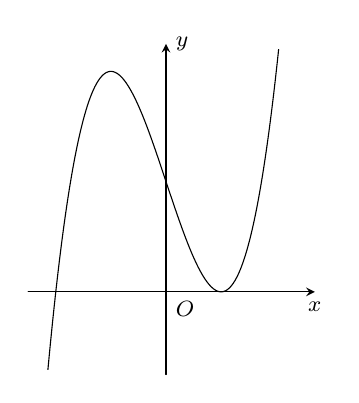
\begin{tikzpicture}[scale=0.7, font=\footnotesize, line join=round, line cap=round,>=stealth]
			\def\a{1} \def\b{0} \def\c{-3} \def\d{2}
			\def\xmin{-2.5} \def\xmax{2.7}
			\def\ymin{-1.5} \def\ymax{4.5} 
			\draw[->] (\xmin,0)--(\xmax,0) node [below]{$x$};
			\draw[->] (0,\ymin)--(0,\ymax) node [right]{$y$};
			\node at (0,0) [below right]{$O$};
			\clip (\xmin+0.1,\ymin+0.1) rectangle (\xmax-0.5,\ymax-0.1);
			\draw[smooth,samples=300] plot(\x,{\a*(\x)^3+\b*(\x)^2+\c*(\x)+\d});
			\tkzDefPoints{0/0/O}
			\tkzDrawPoints[fill=black](O)
		\end{tikzpicture}
	}
	\loigiai{
		Đường cong trên hình là đồ thị của hàm số bậc ba với hệ số $a>0$ nên chỉ có $y=x^3-3x+2$ là đúng.}
\end{ex}

\begin{ex}%[Đề thi thử TN Hà Tĩnh 2023]%[An Le - Ex6]%[2D4B1-1]
	Cho hai số phức $z_1=1-2i$, $z_2=-2+3i$. Phần ảo của số phức $z=z_1 \cdot z_2$ bằng
	\choice
	{$4$}
	{$7i$}
	{\True $7$}
	{$-7$}
	\loigiai{
		Ta có $z=z_1 \cdot z_2 = (1-2i)\cdot (-2+3i)= 4 + 7i$. Suy ra phần ảo của số phức $z$ bằng $7$.
	}
\end{ex}

\begin{ex}%[Đề thi thử TN Hà Tĩnh 2023]%[An Le - Ex6]%[2D1B4-1]
	Cho hàm số $y=\dfrac{2x+1}{x+2}$. Tọa độ giao điểm của hai đường tiệm cận của đồ thị hàm số là
	\choice
	{$(2;2)$}
	{\True $(-2;2)$}
	{$\left( -2;-\dfrac{1}{2} \right)$}
	{$(2;-2)$}
	\loigiai{
		Ta có $\lim \limits_{x \to \pm \infty} \dfrac{2x+1}{x+2}=2$, $\lim \limits_{x \to -2^+} \dfrac{2x+1}{x+2}=-\infty$, $\lim \limits_{x \to -2^-} \dfrac{2x+1}{x+2}=+\infty$.\\
		Do đó, đồ thị hàm số có đường tiệm cận đứng $x=-2$, đường tiệm cận ngang $y=2$ nên toạ độ giao điểm hai đường tiệm cận là $I(-2;2)$.
	}
\end{ex}

\begin{ex}%[Đề thi thử TN Hà Tĩnh 2023]%[An Le - Ex6]%[2D2B6-1]
	Tập nghiệm của bất phương trình $\log_2(x-2) \leq 2$ là
	\choice
	{$(-\infty;6)$}
	{\True $(2;6]$}
	{$(-\infty;6]$}
	{$[2;4]$}
	\loigiai{
		Bất phương trình tương đương với $0<x-2 \leq 4 \Leftrightarrow 2<x \leq 6$.
	}
\end{ex}

\begin{ex}%[Đề thi thử TN Hà Tĩnh 2023]%[An Le - Ex6]%[2D1B1-1]
	Hàm số nào sau đây đồng biến trên khoảng $(-\infty;+\infty)$?
	\choice
	{\True $y=x^3+3x+2$}
	{$y=\dfrac{2x-1}{x+2}$}
	{$y=\dfrac{1}{4}x^4+x^2$}
	{$y=-x^3-x+2$}
	\loigiai{
		Xét hàm số $y=x^3+3x+2$ có $y'=3x^2+3>0,\ \forall x\in\mathbb{R}$.\\
		Vậy hàm số $y=x^3+3x+2$ đồng biến trên khoảng $(-\infty;+\infty)$.
	}
\end{ex}

\begin{ex}%[Đề thi thử TN Hà Tĩnh 2023]%[An Le - Ex6]%[2D3B3-1]
	Diện tích hình phẳng giới hạn bởi parabol $(P)\colon y=x^2+2x$ và đường thẳng $d \colon y=2x+1$ bằng
	\choice
	{$S=\dfrac{4\pi}{3}$}
	{$S=\dfrac{16}{15}$}
	{$S=\dfrac{16\pi}{15}$}
	{\True $S=\dfrac{4}{3}$}
	\loigiai{
		Xét phương trình $x^2+2x=2x+1\Leftrightarrow x^2-1=0\Leftrightarrow x=\pm 1$.\\
		Diện tích cần tình là
		$$S=\displaystyle\int\limits_{-1}^{1} \left|x^2-1\right| \mathrm{\,d}x=\dfrac{4}{3}.$$
	}
\end{ex}

\begin{ex}%[Đề thi thử TN Hà Tĩnh 2023]%[An Le - Ex6]%[1H3B5-3]
	Cho hình chóp $S.ABC$ có đáy là tam giác vuông cân tại $B$, $SA$ vuông góc với đáy và $AB=4$. Khoảng cách từ $C$ đến mặt phẳng $\left(SAB\right)$ bằng
	\choice
	{\True $4$}
	{$2\sqrt{2}$}
	{$4\sqrt{2}$}
	{$8\sqrt{2}$}
	\loigiai{
		\immini
		{
			Ta có $CB\perp AB$, $CB\perp SA$ nên $CB\perp (SAB)$ do đó khoảng cách từ $C$ đến $(SAB)$ là $CB=4$.
		}
		{
			\begin{tikzpicture}[scale=.6,font=\footnotesize, line join=round, line cap=round, >=stealth]
				\tkzDefPoints{0/0/A,5/0/C,2/-2/B}
				\coordinate (S) at ($(A)+(0,5)$);
				\draw (S)--(A)--(B)--(C)--(S)--(B);
				\draw[dashed](A)--(C);
				\foreach \x/\g in {A/180,B/-90,C/0,S/90} \fill[black](\x) circle (1pt) ($(\x)+(\g:3mm)$) node{$\x$};
			\end{tikzpicture}
		}
	}
\end{ex}

\begin{ex}%[Đề thi thử TN Hà Tĩnh 2023]%[An Le - Ex6]%[2D1B5-3]
	\immini
	{
		Cho hàm số bậc ba $y=f(x)$ có đồ thị như hình vẽ bên. Phương trình $\left|f(x)\right|=1$ có bao nhiêu nghiệm thực phân biệt?
	\choice
	{\True $6$}
	{$5$}
	{$4$}
	{$3$}
	}
	{
		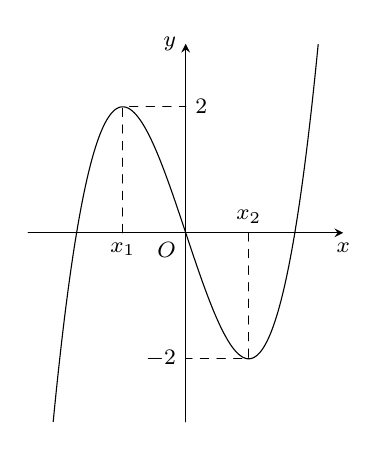
\begin{tikzpicture}[scale=.8,font=\footnotesize, line join=round, line cap=round, >=stealth]
			%%Nhập giới hạn đồ thị và hàm số cần vẽ
			\def \xmin{-2.5}
			\def \xmax{2.5}
			\def \ymin{-3}
			\def \ymax{3}
			\def \hamso{(\x)^3-3*(\x)}
			%\def \tiemcanxien{\x+1}
			%%Tự động
			\draw[->] (\xmin,0)--(\xmax,0) node[below] {$x$};
			\draw[->] (0,\ymin)--(0,\ymax) node[left] {$y$};
			\draw (0,0) node [below left] {$O$};
			\draw[dashed] (-1,0)node[below]{$x_1$}--(-1,2)--(0,2)node[right]{$2$}
			(1,0)node[above]{$x_2$}--(1,-2)--(0,-2)node[left]{$-2$};
			%%Tự động
			\begin{scope}
				\clip (\xmin+0.01,\ymin+0.01) rectangle (\xmax-0.01,\ymax-0.01);
				\draw[samples=350,domain=\xmin+0.01:\xmax-0.01,smooth,variable=\x] plot (\x,{\hamso});
			\end{scope}
		\end{tikzpicture}

	}
	\loigiai{
		\immini
		{
			Phương trình tương đương với $\hoac{& f(x)=1& (1) \\ & f(x)=-1. & (2)}$\\
		Dựa vào đồ thị ta thấy mỗi đường thẳng $y=1$ và $y=-1$ đều cắt đồ thị $f(x)$ tại $3$ điểm phân biệt và $6$ điểm có hoành độ khác nhau.\\
		Do đó mỗi phương trình $(1)$ và $(2)$ đều có $3$ nghiệm phân biệt và $6$ nghiệm khác nhau.\\
		Vậy phương trình ban đầu có $6$ nghiệm phân biệt. 
		}
		{
			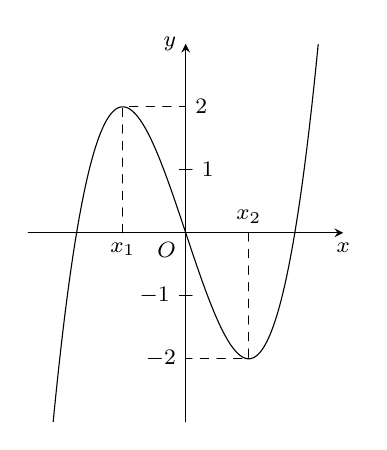
\begin{tikzpicture}[scale=.8,font=\footnotesize, line join=round, line cap=round, >=stealth]
				%%Nhập giới hạn đồ thị và hàm số cần vẽ
				\def \xmin{-2.5}
				\def \xmax{2.5}
				\def \ymin{-3}
				\def \ymax{3}
				\def \hamso{(\x)^3-3*(\x)}
				%\def \tiemcanxien{\x+1}
				%%Tự động
				\draw[->] (\xmin,0)--(\xmax,0) node[below] {$x$};
				\draw[->] (0,\ymin)--(0,\ymax) node[left] {$y$};
				\draw (0,0) node [below left] {$O$}
				(-0.1,1)--(0.1,1)node[right]{$1$}
				(-0.1,-1)node[left]{$-1$}--(0.1,-1);
				\draw[dashed] (-1,0)node[below]{$x_1$}--(-1,2)--(0,2)node[right]{$2$}
				(1,0)node[above]{$x_2$}--(1,-2)--(0,-2)node[left]{$-2$};
				%%Tự động
				\begin{scope}
					\clip (\xmin+0.01,\ymin+0.01) rectangle (\xmax-0.01,\ymax-0.01);
					\draw[samples=350,domain=\xmin+0.01:\xmax-0.01,smooth,variable=\x] plot (\x,{\hamso});
				\end{scope}
			\end{tikzpicture}
		}
	}
\end{ex}

\begin{ex}%[Đề thi thử TN Hà Tĩnh 2023]%[An Le - Ex6]%[2D1B2-1]
	Cho hàm số $y=f(x)$ có đạo hàm $f'(x)=\left(x-2\right)^2\left(x-1\right)^3\left(2x+3\right)\left(x+1\right)$ với mọi $x\in\mathbb{R}$. Điểm cực đại của hàm số là
	\choice
	{$x=2$}
	{\True $x=-1$}
	{$x=1$}
	{$x=-\dfrac{3}{2}$}
	\loigiai{
		Ta có $f'(x)=0\Leftrightarrow\hoac{& x=-\dfrac{3}{2} \\ & x=-1\\ & x=1\\ & x=2.}$\\
		Bảng xét dấu
		\begin{center}
			
\begin{tikzpicture}
				\tkzTabInit[lgt=1.2,espcl=2]
				{$x$ /1, $f’(x)$ /1}
				{$-\infty$,$-\dfrac{3}{2}$,$-1$, $1$,$2$,$+\infty$}
				\tkzTabLine{ ,-,z,+,z,-,z,+,z,+, }
			\end{tikzpicture}
		\end{center}
	Từ bảng xét dấu ta thấy, $f'(x)$ chỉ có một lần đổi dấu từ dương sang âm khi qua $x=-1$.\\ 
	Vậy điểm cực đại của hàm số là $x=-1$.
	}
\end{ex}

\begin{ex}%[Đề thi thử TN Hà Tĩnh 2023]%[An Le - Ex6]%[1D2B5-2]
	Một hộp bút bi gồm $6$ bút màu đỏ khác nhau, $7$ bút màu đen khác nhau và $8$ bút màu xanh khác nhau. Lấy ngẫu nhiên $4$ bút từ hộp đó, xác suất để trong $4$ bút lấy ra, có đúng $1$ bút màu đỏ bằng
	\choice
	{$\dfrac{104}{285}$}
	{\True $\dfrac{26}{57}$}
	{$\dfrac{9}{19}$}
	{$\dfrac{7}{19}$}
	\loigiai{
		Số phần tử của không gian mẫu bằng $n\left(\Omega\right) = \mathrm{C}_{21}^4$.\\
		Trong $4$ bút lấy ra có đúng $1$ bút màu đỏ và $3$ bút còn lại không phải màu đỏ, do đó số kết quả thuận lợi của biến cố bằng $\mathrm{C}_6^1 \cdot \mathrm{C}_{15}^3$.\\
		Xác suất cần tìm bằng $\dfrac{\mathrm{C}_6^1 \cdot \mathrm{C}_{15}^3}{\mathrm{C}_{21}^4} = \dfrac{26}{57}$.
	}
\end{ex}

\begin{ex}%[Đề thi thử TN Hà Tĩnh 2023]%[An Le - Ex6]%[2D2B5-3]
	Tổng tất cả các nghiệm của phương trình $9^x-4\cdot 3^x+3=0$ bằng
	\choice
	{$4$}
	{\True $1$}
	{$3$}
	{$-4$}
	\loigiai{
		Phương trình tương đương với $\heva{& 3^x=1 \\ & 3^x=3} \Leftrightarrow \heva{& x=0 \\ & x=1}$.\\
		Tổng tất cả các nghiệm của phương trình là $0+1=1$.
	}
\end{ex}

\begin{ex}%[Đề thi thử TN Hà Tĩnh 2023]%[An Le - Ex6]%[2D4B2-4]
	Trên mặt phẳng tọa độ, biết tập hợp điểm biểu diễn số phức $z$ thỏa mãn $\left|z+3i\right|=\left| z+1-2i\right|$ là một đường thẳng. Phương trình tổng quát của đường thẳng đó là
	\choice
	{$x+y+3=0$}
	{$x+y-2=0$}
	{\True $x-5y-2=0$}
	{$x-5y-6=0$}
	\loigiai{
		Gọi $M(x;y)$ là điểm biểu diễn số phức $z$, ta có
		\begin{eqnarray*}
			&&\left|x+yi+3i\right|= \left|x+yi+1-2i\right|\\
			&\Leftrightarrow& x^2+(y+3)^2 = (x+1)^2+(y-2)^2\\
			&\Leftrightarrow& x-5y-2=0.
		\end{eqnarray*}
		Vậy PTĐT cần tìm là $x-5y-2=0$.
	}
\end{ex}

\begin{ex}%[Đề thi thử TN Hà Tĩnh 2023]%[An Le - Ex6]%[2H3B2-3]
	Trong KG $Oxyz$, cho hai điểm $M\left(1;-1;-1\right)$ và $N\left(5;5;1\right)$. Mặt phẳng trung trực của đoạn thẳng $MN$ có phương trình là
	\choice
	{$2x+3y+z+12=0$}
	{$3x+2y-12=0$}
	{$3x+2y-24=0$}
	{\True $2x+3y+z-12=0$}
	\loigiai{
		Mặt phẳng trung trực của $MN$ đi qua trung điểm $I$ của $MN$ và có véc-tơ pháp tuyến là $\overrightarrow{MN}$.\\
		Ta có $I(3;2;0)$ và $\overrightarrow{MN}=(4;6;2)$ nên phương trình mặt phẳng trung trực của $MN$ là
		$$4(x-3)+6(y-2)+2(z-0)=0 \Leftrightarrow 2x+3y+z-12=0.$$
	}
\end{ex}

\begin{ex}%[Đề thi thử TN Hà Tĩnh 2023]%[An Le - Ex6]%[2H3B3-5]
	Trong KG $Oxyz$, cho đường thẳng $\Delta \colon \dfrac{x-1}{2}=\dfrac{y+1}{-3}=\dfrac{z-2}{2}$ song song với mặt phẳng $(P)\colon x+2y+2z+3=0$. Khoảng cách giữa đường thẳng $\Delta$ và mặt phẳng $(P)$ bằng
	\choice
	{\True $2$}
	{$\dfrac{2}{3}$}
	{$1$}
	{$\dfrac{1}{\sqrt{3}}$}
	\loigiai{
		Chọn điểm $A\left(1;-1;2\right)\in (\Delta)$.\\
		Vì $\Delta$ song song với $(P)$ nên
		$\mathrm{d}\left(\Delta ,(P)\right)=\mathrm{d}\left(A,(P)\right)=\dfrac{\left|1-2+4+3\right|}{\sqrt{1+4+4}}= 2$.
	}
\end{ex}

\begin{ex}%[Đề thi thử TN Hà Tĩnh 2023]%[An Le - Ex6]%[1H3K5-3]
	Cho hình chóp $S.ABCD$ có chiều cao $SA=a$, đáy là hình vuông cạnh $a$. Tính khoảng cách từ trung điểm $M$ của cạnh $SB$ đến mặt phẳng $\left(SCD\right)$.
	\choice
	{\True $\dfrac{a\sqrt{2}}{4}$}
	{$\dfrac{a\sqrt{2}}{2}$}
	{$a\sqrt{2}$}
	{$\dfrac{a\sqrt{3}}{2}$}
	\loigiai{
		\immini
		{
			Ta có $BM$ cắt $(SCD)$ tại $S$ và $M$ là trung điểm $BS$ nên
			$$\dfrac{\mathrm{d}(M,(SCD))}{\mathrm{d}(B,(SCD))}=\dfrac{MS}{BS}=\dfrac{1}{2}\Rightarrow \mathrm{d}(M,(SCD))=\dfrac{1}{2}\mathrm{d}(B,(SCD)).$$
			Lại có $AB\parallel CD\subset (SCD)\Rightarrow AB\parallel (SCD)$\\
			$\Rightarrow \mathrm{d}(B,(SCD))=\mathrm{d}(A,(SCD))$.\\
			Mặt khác, hạ $AH \perp SD$\quad (1). Ta có
			$$\left\{ \begin{aligned}
			& SA\bot CD \\
			& AD\bot CD \\
			\end{aligned} \right.\Rightarrow CD\bot (SAD)\Rightarrow AH\bot CD\quad (2)$$
			Từ $(1)$ và $(2)$ suy ra $AH \perp (SCD)$ hay $\mathrm{d}\left(A,(SCD)\right) = AH$.
		}
		{
			\begin{tikzpicture}[scale=.7,font=\footnotesize, line join=round, line cap=round, >=stealth]
				\tkzDefPoints{0/0/A,5/0/D,-2/-2/B}
				\coordinate (C) at ($(B)+(D)-(A)$);
				\coordinate (S) at ($(A)+(0,5)$);
				\coordinate (H) at ($(S)!.5!(D)$);
				\coordinate (M) at ($(B)!0.5!(S)$);
				\draw (S)--(B)--(C)--(D)--(S)--(C);
				\draw[dashed] (S)--(A)--(B)
				(D)--(A)--(H);
				\foreach \x/\g in {A/180,B/-120,C/-60,D/0,S/90,H/30,M/150} \fill[black](\x) circle (1.5pt) ($(\x)+(\g:3mm)$) node{$\x$};
			\end{tikzpicture}
		}
	
	\noindent
		Tam giác $SAD$ vuông tại $A$, có $SA=a$, $AD=a$ nên là tam giác vuông cân, do đó $H$ là trung điểm của $SD$ và $AH = \dfrac{a\sqrt{2}}{2}$.\\
		Vậy $\mathrm{d}\left(M,(SCD)\right)= \dfrac{1}{2}AH = \dfrac{a\sqrt{2}}{4}$.
	}
\end{ex}

\begin{ex}%[Đề thi thử TN Hà Tĩnh 2023]%[An Le - Ex6]%[2D2K6-3]
	Có bao nhiêu số tự nhiên $x\in\left[1;2023\right]$ thỏa mãn $3^{\log_4x+\dfrac{1}{2}}+3^{\log_4x-\dfrac{1}{2}}\ge\sqrt{x}$.
	\choice
	{$2022$}
	{$2021$}
	{\True $2023$}
	{$2020$}
	\loigiai{
		Điều kiện $x>0$, đặt $t=\log_4x\Leftrightarrow x=4^t$, ta được
		\begin{eqnarray*}
			&& \sqrt{3}\cdot 3^t+\dfrac{1}{\sqrt{3}}\cdot 3^t\ge 2^t\\
			&\Leftrightarrow& 4\cdot 3^t\ge\sqrt{3}\cdot 2^t\\
			&\Leftrightarrow& \left(\dfrac{3}{2}\right)^t\ge\dfrac{\sqrt{3}}{4}\\
			&\Leftrightarrow& t\ge{\log_{\tfrac{3}{2}}}\dfrac{\sqrt{3}}{4}.
		\end{eqnarray*}
	Vậy $x\ge 4^{\log_{\tfrac{3}{2}}\dfrac{\sqrt{3}}{4}}\approx 0{,}06$, nên có $2023$ số tự nhiên $x\in\left[1;2023\right]$ thỏa mãn.
	}
\end{ex}

\begin{ex}%[Đề thi thử TN Hà Tĩnh 2023]%[An Le - Ex6]%[2D3K1-1]
	Cho hàm số $y=f(x)$ xác định trên $\mathbb{R}\setminus\left\{\dfrac{1}{2}\right\}$ thỏa mãn $f'(x)=\dfrac{1}{2x-1}$, $f(0)=2022$, $f(1)=2023$. Giá trị của $f(2)-f\left(-1\right)$ bằng
	\choice
	{$0$}
	{$-1$}
	{\True $1$}
	{$\ln 4$}
	\loigiai{
		Ta có $\displaystyle\int f'(x)\mathrm{\, d}x=\int{\dfrac{1}{2x-1}\mathrm{\, d}x}=\dfrac{1}{2}\ln\left| 2x-1\right|+C\Rightarrow f(x)=\left\{\begin{aligned}&\dfrac{1}{2}\ln\left(2x-1\right)+C_1,\ \text{khi }x >\dfrac{1}{2}\\ &\dfrac{1}{2}\ln\left(1-2x\right)+C_2,\ \text{khi }x <\dfrac{1}{2}.\end{aligned}\right.$
			\begin{itemize}
				\item Xét trên $\left(-\infty ;\dfrac{1}{2}\right)$, ta có $f(0)=2022\Rightarrow C_2=2022$.
				\item Xét trên $\left(\dfrac{1}{2};+\infty\right)$, ta có $f(1)=2023\Rightarrow C_1=2023$.
			\end{itemize}
		Do đó, $f(x)=\left\{\begin{aligned}&\dfrac{1}{2}\ln\left(2x-1\right)+2023,\ \text{khi }x > \dfrac{1}{2}\\ &\dfrac{1}{2}\ln\left(1-2x\right)+2022,\ \text{khi } x < \dfrac{1}{2}.\end{aligned}\right.$\\
		Vậy $f(3)-f\left(-1\right)=\left(\dfrac{1}{2}\ln 3+2023\right)-\left(\dfrac{1}{2}\ln 3+2022\right)=1$.
	}
\end{ex}

\begin{ex}%[Đề thi thử TN Hà Tĩnh 2023]%[An Le - Ex6]%[2D1K5-3]
	Cho hàm số bậc ba $f\left(x\right)$ có bảng biến thiên như hình vẽ. 
	\begin{center}
		
\begin{tikzpicture}
			\tkzTabInit[lgt=1.2,espcl=2]
			{$x$ /.7, $f’(x)$ /.7, $f(x)$ /2}
			{$-\infty$,$x_1$,$x_2$,$+\infty$}
			\tkzTabLine{ ,+,z,-,z,+, }
			\tkzTabVar{-/$-\infty$,+/$3$,-/$1$,+/$+\infty$}
		\end{tikzpicture}
	\end{center}
	Có bao nhiêu giá trị nguyên của $m$ sao cho đồ thị hàm số $g\left(x\right)=\dfrac{1}{f\left(x\right)-m}$ có đúng ba đường tiệm cận?
	\choice
	{$0$}
	{\True $2$}
	{$1$}
	{$3$}
	\loigiai{
		Với mọi $m$, ta có $\lim\limits_{x\to \pm \infty} g(x)= 0$, suy ra hàm số $y=g(x)$ luôn luôn có đúng một đường tiệm cận ngang là $y=0$.\\
		Do đó đồ thị hàm số có đúng ba đường tiệm cận khi và chỉ khi có đúng hai đường tiệm cận đứng, tức là phương trình $f(x)-m=0$ có hai nghiệm phân biệt.\\
		Dựa vào bảng biến thiên, ta thấy có $2$ giá trị của $m\in\{1;3\}$ thoả mãn bài toán.
	}
\end{ex}

\begin{ex}%[Đề thi thử TN Hà Tĩnh 2023]%[An Le - Ex6]%[2D4K5-1]
	Xét các số phức $z$ thỏa mãn $\left|z-2+3i\right|=2|z+1|$. Gọi $M$ và $m$ lần lượt là giá trị lớn nhất và giá trị nhỏ nhất của $|z|$. Giá trị của $M+m$ bằng
	\choice
	{\True $4\sqrt{2}$}
	{$\sqrt{5}$}
	{$2 \sqrt{2}$}
	{$2\sqrt{5}$}
	\loigiai{
		Đặt $z=x+yi$, $x$, $y \in \mathbb{R}$. Từ giả thiết ta có
		\begin{eqnarray*}
			&& \left|x+yi-2+3i\right| = 2\left|x+yi+1\right|\\
			&\Leftrightarrow& (x-2)^2+(y+3)^2=4\left[(x+1)^2+y^2\right]\\
			&\Leftrightarrow& x^2+y^2+4x-2y-3=0.
		\end{eqnarray*}
		\immini
		{
			Tập hợp các điểm biểu diễn số phức $z$ là đường tròn tâm $I(-2;1)$, bán kính $R=2\sqrt{2}$.\\
		Ta thấy $OI=\sqrt{5}<R$ nên điểm $O$ nằm bên trong đường tròn $(C)$.\\
		Do đó
		\begin{itemize}
			\item $M=\max \left|z\right| = \max\limits_{M \in (C)} OM =OM_1= R+OI$.
			\item $m=\min \left|z\right| = \min\limits_{M \in (C)} OM =OM_2= R-OI$.
		\end{itemize}		
		Vậy $M+m = 2R = 4\sqrt{2}$.
		}
		{
			\begin{tikzpicture}[scale=.55,font=\footnotesize, line join=round, line cap=round, >=stealth]
				\tkzDefPoints{0/0/I,3/0/M_2,2/0/O,-3/0/M_1}
				\tkzDrawCircle[radius](I,M_1)
				\draw (M_1)--(M_2);
				\foreach \x/\g in {I/90,O/90,M_1/180,M_2/0} \fill[black](\x) circle (1.5pt) ($(\x)+(\g:4mm)$) node{$\x$};
			\end{tikzpicture}
		}
	}
\end{ex}

\begin{ex}%[Đề thi thử TN Hà Tĩnh 2023]%[An Le - Ex6]%[2H1K3-1]
	Cho khối hộp chữ nhật $ABCD.A'B'C'D'$ có đáy là hình vuông cạnh bằng $2a$. Gọi $M$, $N$ lần lượt là trung điểm của $AB$ và $B'C'$. Biết rằng góc giữa đường thẳng $MN$ và đường thẳng $AA'$ bằng $30^{\circ}$. Thể tích của khối hộp chữ nhật đã cho bằng
		\choice{\True $4a^3\sqrt{6}$}
	{$\dfrac{a^3\sqrt{6}}{3}$}
	{$\dfrac{4a^3\sqrt{6}}{3}$}
	{$2a^3\sqrt{6}$}
	\loigiai{
		\immini
		{
			Gọi $P$ là trung điểm của $BC$, ta có $NP \parallel AA'$, do đó góc giữa $MN$ và $AA'$ bằng góc giữa $MN$ và $NP$.\\
			Vì tam giác $MNP$ vuông ở $P$, $MP=\dfrac{AC}{2}=a\sqrt{2}$ nên góc giữa $MN$ và $NP$ là góc $\widehat{MNP}$, suy ra
			$$\widehat{MNP}=30^{\circ}\Rightarrow NP = \dfrac{MP}{\tan 30^{\circ}} = a\sqrt{6}.$$
			Vậy thể tích khối hộp đã cho bằng
			$$S_{ABCD}\cdot NP = (2a)^2 \cdot a\sqrt{6}=4a^3\sqrt{6}.$$
		}
		{
			\begin{tikzpicture}[scale=.6,font=\footnotesize, line join=round, line cap=round, >=stealth]
				\tkzDefPoints{0/0/A,5/0/D,-2/-2/B}
				\coordinate (C) at ($(B)+(D)-(A)$);
				\coordinate (A') at ($(A)+(0,5)$);
				\coordinate (B') at ($(A')+(B)-(A)$);
				\coordinate (C') at ($(A')+(C)-(A)$);
				\coordinate (D') at ($(A')+(D)-(A)$);
				\coordinate (M) at ($(B)!0.5!(A)$);
				\coordinate (N) at ($(B')!0.5!(C')$);
				\coordinate (P) at ($(B)!0.5!(C)$);
				\draw (B')--(A')--(D')--(C')--(B')--(B)--(C)--(D)--(D')
				(N)--(P)
				(C)--(C');
				\draw[dashed] (A')--(A)--(B)
				(A)--(D)
				(P)--(M)--(N);
				\foreach \x/\g in {A/180,B/-120,C/-60,D/0,D'/60,A'/120,B'/180,C'/-20,M/150,N/90,P/-90} \fill[black](\x) circle (1.5pt) ($(\x)+(\g:3mm)$) node{$\x$};
			\end{tikzpicture}
		}
	}
\end{ex}

\begin{ex}%[Đề thi thử TN Hà Tĩnh 2023]%[An Le - Ex6]%[2H3K3-2]
	Trong KG $Oxyz$, cho hai đường thẳng $d\colon \dfrac{x-1}{3}=\dfrac{y+2}{1}=\dfrac{z}{1}$; $d'\colon \left\{\begin{aligned}& x=t\\ & y=1+2t\\ & z=-1+t\\ \end{aligned}\right.$. Gọi $\Delta$ là đường thẳng đi qua $M(3;2;1)$, vuông góc với $d$ và cắt $d'$. Khi đó tọa độ giao điểm của $\Delta$ và mặt phẳng $\left(Oyz\right)$ là
	\choice
	{$\left(0;2;1\right)$}
	{$\left(0;-11;1\right)$}
	{\True $\left(0;11;1\right)$}
	{$\left(0;-2;1\right)$}
	\loigiai{
		Gọi giao điểm của $\Delta$ và $d'$ là $N(t;1+2t;-1+t)$.\\
		Khi đó $\overrightarrow{MN}=\left(t-3;2t-1;t-2\right) \ne \overrightarrow{0}$, $\forall t$ là véc-tơ chỉ phương của $\Delta$ và $\overrightarrow{u}=(3;1;1)$ là véc-tơ chỉ phương của $d$.\\
		Vì $\Delta \perp d$ nên $\overrightarrow{MN} \cdot \overrightarrow{u} = 0\Leftrightarrow 3(t-3)+(2t-1)+(t-2)=0 \Leftrightarrow t=2$.\\
		Khi đó $\overrightarrow{MN}=(-1;3;0)$ nên PTĐT $\Delta$ là $\left\{\begin{aligned}& x=3-s \\ & y=2+3s\\&z=1.\end{aligned}\right.$\\
		Giao điểm của $\Delta$ và $(Oyz)$ là điểm có toạ độ $(0;11;1)$.
	}
\end{ex}

\begin{ex}%[Đề thi thử TN Hà Tĩnh 2023]%[An Le - Ex6]%[2H2K1-3]
	Cho hình trụ $(T)$ có $AB$, $CD$ lần lượt là hai đường kính của hai đường tròn đáy của hình trụ và đồng thời vuông góc với nhau. Thể tích khối tứ diện $ABCD$ bằng $10$. Thể tích khối trụ $(T)$ bằng
	\choice
	{\True $15\pi$}
	{$30\pi$}
	{$45\pi$}
	{$60\pi$}
	\loigiai{
		\immini
		{
			Gọi $r$ và $h$ lần lượt là bán kính đáy và chiều cao của hình trụ $(T)$.\\
		Thể tích tứ diện $ABCD$ là
		$$V=\dfrac{1}{6}\cdot AB \cdot CD \cdot \mathrm{d}(AB,CD)\cdot \sin (AB,CD).$$
		Ta có $V=10$, $\mathrm{d}(AB,CD) =h$ và $AB\perp CD$, do đó ta có\\
		$10 = \dfrac{1}{6}\cdot 2r \cdot 2r \cdot h \cdot \sin 90^{\circ} \Rightarrow r^2h=15.$\\
		Vậy thể tích khối trụ $(T)$ bằng $\pi r^2h=15\pi$.
		}
		{
			\begin{tikzpicture}[scale=1,font=\footnotesize, line join=round, line cap=round, >=stealth]
				\tkzDefPoints{0/0/A,3/0/B}
				\coordinate (A') at ($(A)+(0,4)$);
				\coordinate (B') at ($(B)+(0,4)$);
				\coordinate (O') at ($(A')!0.5!(B')$);
				\coordinate (D) at ($(O')+({1.5*cos(90)},{0.5*sin(85)})$);
				\coordinate (C) at ($(O')+({1.5*cos(270)},{0.5*sin(265)})$);
				\draw[dashed] (B) arc(0:180:1.5 cm and 0.5 cm)
				(A)--(B)--(C)--(A)--(D)--(B);
				\draw (B) arc(0:-180:1.5 cm and 0.5 cm)
				(B') arc(0:180:1.5 cm and 0.5 cm)
				(B') arc(0:-180:1.5 cm and 0.5 cm)
				(A)--(A') (B)--(B') (C)--(D);
				\foreach \x/\g in {A/180,B/0,C/55,D/60} \fill[black](\x) circle (1pt) ($(\x)+(\g:2mm)$) node{$\x$};
			\end{tikzpicture}
		}
	}
\end{ex}

\begin{ex}%[Đề thi thử TN Hà Tĩnh 2023]%[An Le - Ex6]%[2D3G3-1]
	\immini
	{
		Cho hàm số bậc ba $y=f(x)=ax^3+bx^2+cx+d$ có đồ thị như hình vẽ. Diện tích hình phẳng giới hạn bởi hai đường $y=f'(x)$ và $g(x)=f''(x)+bx-c$ bằng
	\choice
	{$\dfrac{145}{2}$}
	{\True $\dfrac{25}{2}$}
	{$\dfrac{125}{2}$}
	{$\dfrac{29}{2}$}
	}
	{
		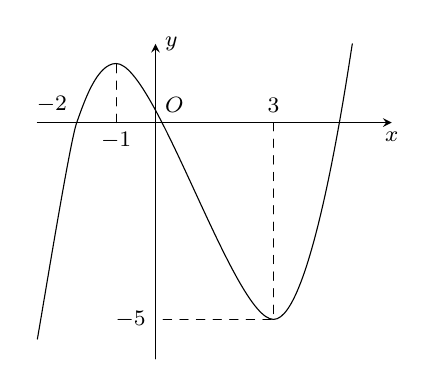
\begin{tikzpicture}[scale=.5,font=\footnotesize, line join=round, line cap=round, >=stealth]
		\def \xmin{-3}
		\def \xmax{6}
		\def \ymin{-6}
		\def \ymax{2}
		\draw[->] (\xmin,0)--(\xmax,0) node[below] {$x$};
		\draw[->] (0,\ymin)--(0,\ymax) node[right] {$y$};
		\draw (0,0) node [above right] {$O$};
		\coordinate (A) at (-3,-5.5);
		\coordinate (B) at (-1,1.5);
		\coordinate (C) at (3,-5);
		\coordinate (D) at (5,2);
		\coordinate (E) at (-2,0);
		\draw 
		(A) .. controls +(80:1) and +(250:.5) .. 
		(E) .. controls +(70:.5) and +(180:.5) .. 
		(B) .. controls +(0:1) and +(180:1) .. 
		(C) .. controls +(0:1) and +(260:.5) .. 
		(D); 
		\draw[dashed] (-1,0)node[below]{$-1$}--(B)
		(3,0)node[above]{$3$}--(C)--(0,-5)node[left]{$-5$}
		(E)node[above left]{$-2$};
		\tkzDrawPoints[fill=black](B,C,E)
	\end{tikzpicture}

	}
	\loigiai{
		Ta có $y'=3ax^2+2bx+c$.\\
		Đồ thị hàm số đi qua điểm $(-2;0)$, $(3;-5)$ và hàm số đạt cực trị tại $x=-1$ và $x=3$ nên ta có hệ phương trình
		$$\begin{aligned}\left\{\begin{aligned}& -8a+4b-2c+d=0 \\ & 27a+9b+3c+d=-5\\&3a-2b+c=0\\&27a+6b+c=0\end{aligned}\right. \Leftrightarrow \left\{\begin{aligned}& a=\dfrac{1}{5} \\ & b=-\dfrac{3}{5}\\&c=-\dfrac{9}{5}\\&d=\dfrac{2}{5}.\end{aligned}\right.\end{aligned}$$
		Khi đó $f(x) = \dfrac{1}{5}x^3-\dfrac{3}{5}x^2-\dfrac{9}{5}x+\dfrac{2}{5}$; $f'(x)=\dfrac{3}{5}x^2-\dfrac{6}{5}x-\dfrac{9}{5}$; $f''(x) = \dfrac{6}{5}x-\dfrac{6}{5}$ và $g(x) = \dfrac{3}{5}x+\dfrac{3}{5}$.\\
		Phương trình hoành độ giao điểm của $f'(x)$ và $g(x)$
		$$\dfrac{3}{5}x^2-\dfrac{6}{5}x-\dfrac{9}{5}=\dfrac{3}{5}x+\dfrac{3}{5}\Leftrightarrow \left[\begin{aligned}& x=-1 \\ & x=4.\end{aligned}\right.$$
		Diện tích hình phẳng giới hạn bởi hai đường $f'(x)$ và $g(x)$ bằng\\
		$$\displaystyle\int\limits_{-1}^4 \left|\dfrac{3}{5}x^2-\dfrac{9}{5}x-\dfrac{12}{5}\right| \mathrm{\,d}x=\dfrac{25}{2}.$$
	}
\end{ex}

\begin{ex}%[Đề thi thử TN Hà Tĩnh 2023]%[An Le - Ex6]%[2D4G4-1]
	Trên tập hợp các số phức, xét phương trình $z^4+2(m+2)z^2+3m+2=0$, ($m$ là tham số thực). Có bao nhiêu giá trị của tham số $m$ sao cho phương trình đã cho có bốn nghiệm phân biệt và bốn điểm $A$, $B$, $C$, $D$ biểu diễn bốn nghiệm đó trên mặt phẳng phức tạo thành một tứ giác có diện tích bằng $4$?
	\choice
	{$0$}
	{$2$}
	{\True $1$}
	{Vô số}
	\loigiai{
		Đặt $t=z^2$, phương trình trở thành $t^2+2(m+2)t+3m+2=0$. \hfill (1)\\
		Ta có, $\Delta ' = (m+2)^2-(3m+2)=m^2+m+2 >0$ ($\forall m \in \mathbb{R}$) nên (1) luôn có hai nghiệm thực phân biệt.
		\begin{itemize}
			\item Nếu (1) có hai nghiệm thực dương hoặc hai nghiệm thực âm thì bốn điểm $A$, $B$, $C$, $D$ thẳng hàng (cùng thuộc $Ox$ hoặc cùng thuộc $Oy$) nên không thoả mãn bài toán.
			\item Nếu (1) có hai nghiệm trái dấu $t_1<0<t_2$, tức là $3m+2<0 \Leftrightarrow m <-\dfrac{2}{3}$ thì phương trình đã cho có 4 nghiệm phân biệt là $\pm \sqrt{t_2}$ và $\pm i \sqrt{-t_1}$.\\
			Giả sử $A\left(-\sqrt{t_2};0\right)$, $B\left(0;\sqrt{-t_1}\right)$, $C\left(\sqrt{t_2};0\right)$ và $D\left(0;-\sqrt{-t_1}\right)$. Khi đó, $AC\perp BD$.\\
			Diện tích $ABCD$ bằng $ \dfrac{1}{2}\cdot AC \cdot BD =\dfrac{1}{2} \cdot 2\sqrt{t_2}\cdot 2\sqrt{-t_1}=2\sqrt{-t_1t_2}.$\\
			Từ giả thiết và theo định lý Vi-ét, ta có
			$2\sqrt{-3m-2}=4 \Leftrightarrow m =-2$.\\
			Đối chiếu điều kiện, ta có $m=-2$ là giá trị cần tìm.
		\end{itemize}
		
	}
\end{ex}

\begin{ex}%[Đề thi thử TN Hà Tĩnh 2023]%[An Le - Ex6]%[2D1G5-5]
	Cho các số thực dương $x$ và $y$ thỏa mãn $4+3^{2x^2-y+2}=\left(4+9^{2x^2-y}\right)\cdot 7^{y-2x^2+2}$. Khi biểu thức $P=\dfrac{x+y+10}{x}$ đạt giá trị nhỏ nhất thì tổng $x+y$ bằng
	\choice
	{$9$}
	{$1+9\sqrt{2}$}
	{\True $8$}
	{$1+8\sqrt{2}$}
	\loigiai{
		Ta có
		\begin{eqnarray*}
			&& 4+3^{2x^2-y+2}=\left(4+9^{2x^2-y}\right)\cdot{7^{y-2x^2+2}}\\
			&\Leftrightarrow & 7^{2x^2-y}\left(4+9\cdot 3^{2x^2-y}\right)=49\left(4+9^{2x^2-y}\right)\\
			&\Leftrightarrow & 4\cdot 7^{2x^2-y}+9\cdot 21^{2x^2-y}-49\cdot 9^{2x^2-y}-196=0.\quad (*)
		\end{eqnarray*}
		Đặt $t=2x^2-y$, $(*)$ trở thành 
		$$4\cdot7^t+9\cdot{21^t}-49\cdot9^t-196=0\Leftrightarrow\dfrac{4+3^{t+2}}{7^{t+2}}=\dfrac{4+3^{2t}}{7^{2t}}.$$
		Xét hàm số $f(a)=\dfrac{4+3^a}{7^a}=4\cdot{\left(\dfrac{1}{7}\right)^a}+\left(\dfrac{3}{7}\right)^a$ là hàm số nghịch biến trên $\mathbb{R}$.\\
		Do đó $(*)\Leftrightarrow f(t+2)=f(2t)\Leftrightarrow t+2=2t\Leftrightarrow t=2\Leftrightarrow 2x^2-y=2$.\\
		Khi đó $P=\dfrac{2x^2+x+8}{x}=2x+\dfrac{8}{x}+1\ge 2\sqrt{2x\cdot\dfrac{8}{x}}+1=9$.\\
		Vậy $P_{\min}=9$ khi $x=2$ và $y=6$, hay $x+y=8$.
	}
\end{ex}

\begin{ex}%[Đề thi thử TN Hà Tĩnh 2023]%[An Le - Ex6]%[2H3G1-3]
	Trong KG $Oxyz$, cho mặt cầu $(S)$ có tâm $I\left(1;2;3\right)$, bán kính $R=5$ và điểm $P\left(2;4;5\right)$ nằm bên trong mặt cầu. Qua $P$ dựng 3 dây cung $AA'$, $BB'$, $CC'$ của mặt cầu $(S)$ đôi một vuông góc với nhau. Dựng hình hộp chữ nhật có ba cạnh là $PA$, $PB$, $PC$. Gọi $PQ$ là đường chéo của hình hộp chữ nhật đó. Biết rằng $Q$ luôn chạy trên một mặt cầu cố định. Bán kính của mặt cầu đó bằng
	\choice
	{\True $\sqrt{57}$}
	{$\sqrt{61}$}
	{$\dfrac{\sqrt{219}}{6}$}
	{$\dfrac{\sqrt{219}}{2}$}
	\loigiai{
		Gọi $G$ là trọng tâm tam giác $ABC$, ta có $3R^2=IA^2+IB^2+IC^2=3IG^2+GA^2+GB^2+GC^2.$\quad	(1)\\
		Lại có $9PG^2=PQ^2=PA^2+PB^2+PC^2=3PG^2+GA^2+GB^2+GC^2.$\quad (2)\\
		Từ (1) và (2) ta có $3R^2=3IG^2+6PG^2\Leftrightarrow IG^2+2PG^2=R^2.$\\
		Vì $\overrightarrow{GQ}+2\overrightarrow{GP}=\overrightarrow{0}$ nên ta có $3\overrightarrow{IG}=\overrightarrow{IQ}+2\overrightarrow{IP}$. Suy ra
		\begin{eqnarray*}
			9IG^2 & = & IQ^2+4IP^2+4 \overrightarrow{IQ}\overrightarrow{IP}\\
			& = & IQ^2+4IP^2+2\left(IQ^2+IP^2-PQ^2\right)\\
			& = & 3IQ^2+6IP^2-2PQ^2\\
			& = & 3IQ^2+6IP^2-18PG^2.
		\end{eqnarray*}
	Do đó, $9IG^2+18PG^2=3IQ^2+6IP^2\Rightarrow IQ^2=3R^2-2IP^2=57$.\\
		Vậy điểm $Q$ luôn di động trên mặt cầu cố định có tâm $I$, bán kính bằng $\sqrt{57}$.
	}
\end{ex}

\begin{ex}%[Đề thi thử TN Hà Tĩnh 2023]%[An Le - Ex6]%[2D1G5-5]
	Cho hàm số $y=f(x)$ có $f(-2)=0$, có đạo hàm liên tục trên $\mathbb{R}$ và bảng xét dấu đạo hàm như sau
	\begin{center}
		
\begin{tikzpicture}
			\tkzTabInit[lgt=1.2,espcl=2]
			{$x$ /.7, $f’(x)$ /.7}
			{$-\infty$,$-1$,$2$,$+\infty$}
			\tkzTabLine{ ,+,z,-,z,+, }
		\end{tikzpicture}
	\end{center}
	Hàm số $g(x)=\left| 3f\left(-x^4+2x^2-2\right)-2x^6+6x^2\right|$ có bao nhiêu điểm cực trị?
	\choice
	{$3$}
	{$4$}
	{\True $5$}
	{$7$}
	\loigiai{
		Đặt $h(x)=3f\left(-x^4+2x^2-2\right)-2x^6+6x^2$.\\
		Ta có $h'(x)=-12x\left(x^2-1\right)\left[f'\left(-x^4+2x^2-2\right)+x^2+1\right]$.\\
		Mà $-x^4+2x^2-2=-\left(x^2-1\right)^2-1\le-1,\forall x\in\mathbb{R}$.\\
		Nên dựa vào bảng xét dấu của $f'(x)\Rightarrow f'\left(-x^4+2x^2-2\right)\ge 0\Rightarrow f'\left(-x^4+2x^2-2\right)+x^2+1>0,\forall x\in\mathbb{R}$.\\
		Do đó dấu của $h'(x)$ cùng dấu với $u(x)=-60x\left(x^2-1\right)$, tức là đổi dấu khi đi qua các điểm $x=-1$; $x=0$; $x=1$.\\
		Vậy hàm số $h(x)$ luôn có 3 điểm cực trị.\\
		Ta có $h(0)=3f(-2)=0$ nên đồ thị hàm số $y=h(x)$ tiếp xúc trục hoành tại $O$ và cắt trục hoành tại $3$ điểm phân biệt.\\
		Vậy $y=g(x)$ có $5$ điểm cực trị.
	}
\end{ex}

\Closesolutionfile{ans}
\begin{indapan}{10}
	{ans/ans-2-TT-26-SGDHaTinh-23}
\end{indapan}